%!TEX root = ../article.tex


%%%%%%%%%%%%%%%%%%%%%%%%%%%%%%%%%%%%%%%%%%%%%%%%%%%%%%%%%%%%%%%%%%%%%%%%%%%%%%%
%%%%%%%%%%%%%%%%%%%%%%%%%%%%%%%%%%%%%%%%%%%%%%%%%%%%%%%%%%%%%%%%%%%%%%%%%%%%%%%
\section{Introduction}
\label{sec:introduction}
%%%%%%%%%%%%%%%%%%%%%%%%%%%%%%%%%%%%%%%%%%%%%%%%%%%%%%%%%%%%%%%%%%%%%%%%%%%%%%%
%%%%%%%%%%%%%%%%%%%%%%%%%%%%%%%%%%%%%%%%%%%%%%%%%%%%%%%%%%%%%%%%%%%%%%%%%%%%%%%

% Let us remind first the famous Pythagoras' theorem:

% \begin{align}\label{eq:pythagore}
% 	\norm{x+y}^2 = \norm{x}^2 + \norm{y}^2 \enspace.
% \end{align}

% Note that \Cref{eq:pythagore} is ok only under some conditions.
% In terms of visualisation, you can reference a figure easily using the command \Cref{fig:pythagore} or using Fig.~\ref{fig:pythagore}.

% \begin{figure}[h] % h stands for here
% 	\centering
% 	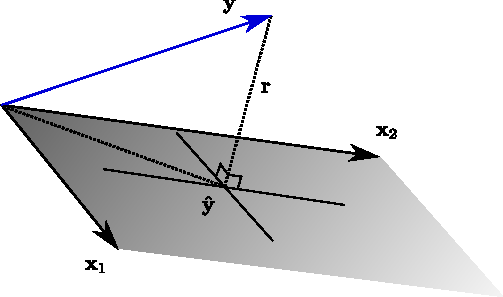
\includegraphics[width=0.6\textwidth]{residu_orth}
% 	\caption{Illustration of the residual orthogonality in least-squares.}
% 	\label{fig:pythagore}
% \end{figure}


% Also an image that is in the \texttt{prebuiltimages/} directory can also be loaded the same way:

% \begin{figure}[h] % h stands for here, ! forces even more...
% 	\centering
% 	
\includegraphics[width=0.2\textwidth]{umontpellier_logo}
% 	\caption{Illustration of a prebuiltimage available.}
% 	\label{fig:umontpellier_logo}
% \end{figure}


% For displaying side by side some images one should consider the package \lstinline+subcaptions+, that can be loaded with the \LaTeX command:

% \begin{lstlisting}[language=tex]
% \usepackage{subcaption}
% \end{lstlisting}


% \begin{figure}[t] % t stands for top (up!)
%     \centering
%     \begin{subfigure}[b]{0.33\textwidth}
%     	\centering
%         
\includegraphics[width=0.2\textwidth]{umontpellier_logo}%
%         \caption{First example}
%         \label{subfig:pythagore}
%     \end{subfigure}
%     \begin{subfigure}[b]{0.56\textwidth}
%     	\centering
%         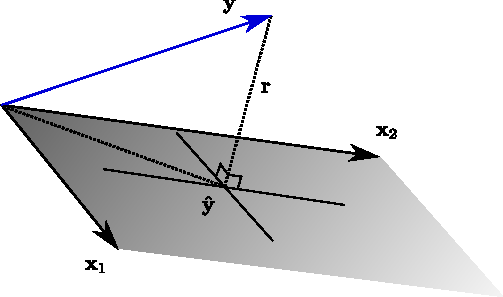
\includegraphics[width=0.5\textwidth]{residu_orth}%
%         \caption{Second example}
%         \label{subfig:logo}
%     \end{subfigure}
%     \caption{Exemples of side by side images}
%     \label{fig:double_example}
% \end{figure}

\textcolor{red}{DRAFT}

Magneto-/electroencephalography (M/EEG) allows for a non-invasive analysis of
functional brain imaging. The distributed-source approach models the brain activity
with a fixed number of dipoles distributed over a dense three-dimensional 
grid within the brain volume. The task in the inverse problem  is to estimate the 
distribution of dipolar currents that can explain the measured data. Since the 
number of dipoles is typically much larger than the number of sensors placed on 
the skull surface of the subject, source localization is an ill-posed inverse problem. 
This implies that there is not a unique solution and that constraints need to be 
applied on the solution. Those constraints must enforce biological assumptions 
made on the brain activity namely, group sparsity and stationarity.
\\
Literature exhibits a large number of techniques such as sparse Bayesian modeling 
(\textcolor{red}{REFERENCE}) and regularized regression (\textcolor{red}{REFERENCE}) 
to model brain activity. In this paper, we are particularly interested in the 
high-dimensional regression setting using group-Lasso-like structured sparsity. 
Those models are usually parametrized by one or multiple hyperparameters to 
control the level of sparsity induced by the constraint.
\\
Hyperparameter selection remains a challenging task, especially in the source 
localization setting. A naive approach consists in selecting the hyperparameters 
by cross-validation (CV). However, the CV approach requires the i.i.d. assumption 
to be fulfilled, which is often not the case when dealing with array of sensors 
(\textcolor{red}{REFERENCE}). Another approach consists in using a hierarchical 
Bayesian model and estimating the hyperparameters by maximum-a-posteriori 
(\textcolor{red}{REFERENCE}). Those approaches still require the tuning of one
or multiple parameters to parametrize hyperpriors.
\\
In this paper, we study the multi-task Lasso problem. In particular, we focus 
our study both on its convex form using a $\ell_{2, 1}$ penalization and its non-convex 
form using a $\ell_{2, 0.5}$ penalization. First, we review the SURE-based approaches
for hyperparameter selection in the neuro-imaging context. Then, we propose a 
procedure based on the Monte-Carlo finite difference SURE \cite{Deledalle_Vaiter_Fadili_Peyre14}
for M/EEG source localization problem that exhibits good performance while being
fast. An implementation of our code can be found in MNE software (\textcolor{red}{REFERENCE}).
The different strategies are tested on simulations and multiple source reconstruction 
problems using public M/EEG data.
\\
\\
\textit{\textbf{Notation}} The transpose of a matrix $\mathbf{A} \in \mathbb{R}^{M \times N}$ is
denoted $\bf{A}^\top$. $\mathbf{A}[i,:]$ and $\mathbf{A}[:,j]$ correspond to the $i^{th}$
row and the $j^{th}$ column respectively. $\norm{A}_{\text{F}}$ indicates the Frobenius norm,
and $\norm{\mathbf{A}}_{p,q}$ the $\ell_{p,q}$ mixed norm with $\norm{\mathbf{A}}_{p,q} 
= \left(\sum_i \left(\sum_j \lvert \mathbf{A}[i,j] \rvert^p\right)^{q/p}\right)^{1/q}$.
$\mathbf{I}$ denotes the identity matrix.


\textcolor{blue}{TODO}
\begin{itemize}
    \item Ill-posed MEEG inverse problem
    \item Prior Lasso Fast solvers for sparse regression
    \item How to select the hyperparameter?
    \item Cross-validation? SURE?
    \item (Fig avec plusieurs valeurs des hyperparams?)
\end{itemize}
%
% \textcolor{blue}{TODO contributions}
In this paper the propose:
\begin{itemize}
    \item New contribution 1
    \item New contribution 2
\end{itemize}

%%%%%%%%%%%%%%%%%%%%%%%%%%%%%%%%%%%%%%%%%%%%%%%%%%%%%%%%%%%%%%%%%%%%%%%%%%%%%%%
\subsection{Background}
\label{sub:background}
%%%%%%%%%%%%%%%%%%%%%%%%%%%%%%%%%%%%%%%%%%%%%%%%%%%%%%%%%%%%%%%%%%%%%%%%%%%%%%%
%

\subsubsection{The multi-task Lasso regression model}

The linear problem can be written as:

\begin{equation}
    \mathbf{M = GX + E} 
\end{equation}
%
where $\mathbf{M} \in \mathbb{R}^{N \times T}$ is a measurement matrix where $N$ is the
number of sensors placed on the skull surface and $T$ is the number of time instants.
$\mathbf{G} \in \mathbb{R}^{N \times S}$ is the design matrix, a known 
instantaneous mixing matrix also called the gain matrix. This matrix relates the source
to the measurements. $\mathbf{E} \in \mathbb{R}^{N \times T}$ is the noise matrix, which
is assumed to be additive, white and Gaussian, $\mathbf{E}[:,j] \sim \mathcal{N}(0, \mathbf{I})
\enspace \forall j$. $\mathbf{X} \in \mathbf{R}^{S \times T}$ is the coefficient matrix to be estimated. 
It corresponds at every point in time to the estimated current intensity in the dipoles of
the brain volumes.
\\
Assuming a known regularization parameter $\lambda > 0$, we recall the multi-task
Lasso regression model defined by:

\begin{equation}
    \mathbf{X}_{\lambda}^* = \argmin_{\mathbf{X}}
    \frac{1}{2}\norm{\mathbf{M - GX}}^2_{\text{F}}
    + \lambda \mathcal{P}(\mathbf{X})
    \enspace ,
\end{equation}
%
where $\mathcal{P}(\mathbf{X})$ is a regularization term and $\lambda$ the hyperparameter
that controls the trade-off between the data-fit and the penalization. In practice, the solution
$\hat{\mathbf{X}}_{\lambda}$ relies heavily on $\lambda$.

\subsubsection{The bi-level optimization framework}

The hyperparameter selection problem can be cast in a bi-level optimization framework (see ???
for a comprehensive review of hyperparameter selection). We will denote $\mathcal{L}$ the cost function
(e.g. a SURE-based criterion), often referred to as the outer loss. Therefore, we can naturally write
the hyperparameter optimization problem as the nested bi-level optimization problem:

\begin{align*}
    &\lambda^* = \argmin_{\lambda} 
    \Biggl\{
        \mathcal{L}(\lambda) 
        \triangleq 
        \mathcal{C}(\mathbf{X}_{\lambda}^*)
    \Biggr\} \\
    &\text{s.t.} \quad 
    \mathbf{X}_{\lambda}^* 
    \in 
    \argmin_{\mathbf{X}} L(\mathbf{X}, \lambda)
    \enspace ,
\end{align*}
%
where $L$ is a convex or non-convex loss function of the coefficient matrix $\mathbf{X}$, 
often referred as the inner loss.

\subsubsection{SURE, a surrogate of the quadratic risk}

\begin{itemize}
    \item Optimization problems (non-convex)
    \item Problem bilevel de la crossval
    \item Dire en detail pq la crossval "c'est pas bien", donner un exemple
    \item SURE: expliquer pourquoi le SURE et les différentes techniques d'approx du SURE
\end{itemize}
%
%
%
%
%%%%%%%%%%%%%%%%%%%%%%%%%%%%%%%%%%%%%%%%%%%%%%%%%%%%%%%%%%%%%%%%%%%%%%%%%%%%%%%
\subsection{Experience}
\label{sub:experience}
%%%%%%%%%%%%%%%%%%%%%%%%%%%%%%%%%%%%%%%%%%%%%%%%%%%%%%%%%%%%%%%%%%%%%%%%%%%%%%%
%

\clearpage
